\documentclass[twocolumn]{article}

\usepackage{graphicx}
\usepackage{xeCJK}
\usepackage{bm}
\usepackage{amsmath,amsthm,amssymb,amsfonts}
\usepackage{cite}
\usepackage[colorlinks,linkcolor=red,anchorcolor=blue,citecolor=green,CJKbookmarks=true]{hyperref}
\usepackage{indentfirst}
\usepackage{amsmath}
\usepackage[margin=3.5cm]{geometry}
\usepackage{titlesec}
\usepackage{amsmath}
\usepackage{amssymb}
% \linespread{1.6}
\usepackage{multirow}
\usepackage{listings}
\usepackage{xcolor}
\usepackage{ulem}
\geometry{left=1.8cm,right=1.8cm,top=1.5cm,bottom=1.5cm}
\usepackage{enumitem}
\usepackage{tikz}
\usepackage{lipsum}
\setenumerate[1]{itemsep=0pt,partopsep=0pt,parsep=\parskip,topsep=5pt}
\setitemize[1]{itemsep=0pt,partopsep=0pt,parsep=\parskip,topsep=5pt}
\setdescription{itemsep=0pt,partopsep=0pt,parsep=\parskip,topsep=5pt}
%定理
\makeatletter
\thm@headfont{\sc}
\makeatother
\newtheorem{theorem}{Theorem}
%%%%%%%%%%%%% C++ Code
\usepackage{color}
\usepackage{xcolor}
\definecolor{keywordcolor}{rgb}{0.8,0.1,0.5}
\usepackage{listings}
\lstset{breaklines}%这条命令可以让LaTeX自动将长的代码行换行排版
\lstset{extendedchars=false}%这一条命令可以解决代码跨页时,章节标题,页眉等汉字不显示的问题
\lstset{ %用于设置语言为C++
    keywordstyle=\color{keywordcolor} \bfseries, 
    %identifierstyle=,
    basicstyle=\ttfamily, 
    commentstyle=\color{blue} \textit,
    stringstyle=\ttfamily, 
    showstringspaces=false,
    frame=shadowbox, %边框
    %captionpos=b
}

%\setCJKmainfont[BoldFont = 黑体]{宋体}
\setlength{\parindent}{2em}
%如果不要缩进 用\noindent
\title{\textbf{An Implementation of SAT-Based Two-Terminal \\ Path Finding Using Z3 Solver}}

\author{YiHong Gu \\ Tsinghua University \\ Beijing, China \\ gyh15@mails.tsinghua.edu.cn}

\date{}

\begin{document}

\maketitle

\section{Introduction}

The 'Two-Terminal Path Finding Problem' has the following description: given $N \times N$ routing grids, and $M$ pairs of terminals, you should use program to find routing paths connecting each pair of terminals. The limit is that different paths cannot cross each other, and no path can cross obstacles. The objective is to maxmize the number of connected pairs, and when all pairs of terminals can be connected, you should minimize the total length of all the paths.

In order to make the objective more clear and not change the original idea of the problem, we simply make the following stipulates that if one grid is defined to be one terminal of pair $d$, then other pairs $d'(d \neq d')$ can not route across the grid.

\section{Related Work}

\cite{source1} gives a general routing methodology which mainly uses 3 kinds of variable as parameters and use Z3 solver to solve the problem. The abstract idea is that giving a concrete illustration of each pairs: for each pair, define a droplet that starts from the origin and ends in terminal during time $t^*$ and $t^\dagger$, and then define the binary variable $c_{p,d}^t$ to illustrate whether the droplet $d$ is at the position $p$ in time $t$. It sets a lot of limits to ensure that (1) each droplet $d$ appears in the board during time $t^*_d$ to time $t^\dagger_d$ and it is at its origin position $p^*_d$ in time $t^*_d$ and at its terminal position $p^\dagger_d$ in time $t^\dagger_d$ (2) every second each droplet only appears at one position (3) the droplet satisfy the routing rule that can only step to one adjacent position per second.

Z3 solver\cite{source2}, developed by Microsoft Research, can use optimized algorithm to check whether it can satisfy all constraints and give a concrete solution. Moreover, it can also maximize/minimize one single variable or expression under all constraints.

\section{SAT-Based Model}

This part is divided into three main parts, sperately illustrate three different models: the original model which resembles the model established in\cite{source1}, the model which resembles network flow, the model which combined the 2 models above.

In the beginning, we just emphasize the definitions:

\begin{itemize}
	\item $N$: the size of the routing boards.
	\item $M$: number of pairs.
	\item $d$: the index of one single droplet.
	\item $t$: the time.
	\item $p$: one single position, can be represented by $p = (x, y) \in \{1, \cdots, N\} \times \{1, \cdots, N\}$.
	\item $P$: the set of all $p$.
	\item $B(p)$: the set of positions that are adjacent to the position $p$ in four direction(up, down, left, right).
	\item $p^*_d$, $p^\dagger_d$: the origin and terminal of droplet $d$.
\end{itemize}

\subsection{Model 1: Based on the Paper}

We use the notation that resembles the original notation in \cite{source1}, and define the binary variable $c_{p,d}^t$ to illustrate whether the droplet $d$ is at the position $p$ in time $t$, and the constraints can be divided into four main parts:

\textbf{to be or not to be}: we can simplify the $t^*$ and $t^\dagger$ and assume every droplet appears at the board in time $1$ (if we want to connect the two-terminal pair), so the constraints can be (for each $d$):

\[
 c_{p^*_d,d}^1 \to \bigvee_{t=1}^{T} c_{p^*_d, d}^t
\]

It means: if it appears, then it must reach the terminal.

\textbf{second conflict}: it means every second each droplet only appears at one position, so the constraints can be (for each $d$):

\[
\bigwedge_{t=1}^{T} \bigwedge_{p \in P} \bigwedge_{p' \in P, p' \neq p} \neg c_{p, d}^t \vee \neg c_{p', d}^t
\]

\textbf{position conflict} firstly every grid can only be visited once (for each $p$)

\[
\bigwedge_{d=1}^{M} \bigwedge_{d'=d+1}^{M} \bigwedge_{t=1}^{T}  \bigwedge_{t'=t+1}^{T} \neg c_{p, d}^t \vee \neg c_{p, d'}^{t'}
\]

\[
\bigwedge_{d=1}^{M} \bigwedge_{t=1}^{T}  \bigwedge_{t'=t+1}^{T} \neg c_{p, d}^t \vee \neg c_{p, d}^{t'}
\]

Also, for each position $p$ which has obstacles for droplet $d$, for all $t$, $c_{p, d}^t$ must be FALSE.

\textbf{travel constraints}: it means the droplet satisfy the routing rule that can only step to one adjacent position per second. So for each droplet $d$, if it appears at position $p$ in time $t$, it must appears at the adjacent position $p'$ in time $t-1$ (except $t=1$).

\[
c_{p, d}^t \to (\bigvee_{p' \in B(p)} c_{p', d}^{t-1})
\]

\textbf{optimization object}: if we want to maxmize the total pairs, we just need to maxmize

\[
\sum_{d=1}^{M}{[c_{p^*_d,d}^1]}
\]

If we want to minmize the total length, we firstly enforce that every $c_{p^*_d,d}^1$ should be TRUE and then minimize

\[
\sum_{d}\sum_{p}\sum_{t}{[c_{p,d}^t]}
\]

Note that the notation

\[
[statement] = \begin{cases} 1, &statement = TRUE\cr 0, &statement = FALSE\end{cases}
\]

We can find the scale of the variables and the constraints are very large, we have totally $T \times N^2 \times M^2$ variables and almost $O(T^2 N^4 M^2)$ contraints, which $T$ represents the maximum time used and it can be $\frac{N^2}{2}$ under the worst condition. If we simply make $N$ be $10$, $M$ be $4$, we can't afford to work it out by our personal computer.

\subsection{Model 2: Based on the Network Flow}

In this model, we directly use the model resembles network flow architecture, for each droplet $d$, we build a network flow graph and set the source to be the origin and sink to be the terminal, and all the positions must satisfy the flow conservation. Then we have $M$ layers network flow graph, afterwards we implement the constraint that every position can be only visited once using a constraint like linear constraint.

In this model, if we use some artifice, we can only have totally $2 \times N^2 \times M$ variables and $O(\times N^2 \times M)$ contraints. Besides, after a large quantity of attempts we find if we conbine several contraints together, we can accelerate the speed of our algorithm, and this things can be concretely described in the next section.

\subsection{Model 3: The Mixed One}

Combine model 1 and model 2 together, we can find a more efficient model, which only have $N^2 \times M$ variables and is 1.5 times faster than model 2.

We use the binary variable $c_{p,d}$ to represent whether the droplet $d$ visit across the position $p$, therefore the contraints are as follows:

\textbf{limit terms} if it is a barrier or is not in the corresponding layer, we enforce $c_{p,d}$ to be FALSE, also we force that every position can only be visited once by the following contraint (for each $p$)

\[
\sum_{d=1}^{M} [c_{p,d}] \le 1
\]

\textbf{source and sink terms}: for each $d$, we come up with a contraint that

\[
c_{p^*_d,d} \leftrightarrow c_{p^\dagger_d,d}
\]

\textbf{connection terms}: for each $p$ which is not the terminal/origin/obstacle grid, it must satisfy the following contraint for each $d$:

\[
c_{p,d} \to (\sum_{p' \in B(p)}c_{p',d} = 2)
\]

and for each $p$ which is equal to $p^*_d$ or $p^\dagger_d$ for a specific $d$, it must satisfy the following contraint:

\[
c_{p,d} \to (\sum_{p' \in B(p)}c_{p',d} = 1)
\]

\textbf{optimization object}: if we want to maxmize the total pairs, we just need to maxmize

\[
\sum_{d=1}^{M}{[c_{p^*_d,d}]}
\]

If we want to minmize the total length, we firstly enforce that every $c_{p^*_d,d}$ should be TRUE and then minimize

\[
\sum_{d}\sum_{p}{[c_{p,d}]}
\]

\section{Optimization}

However, the models above don't have efficiency when the graph is sparse. For example, for a board that $N=10$, if we set $M=9$ and place the 9 pairs over the whole board, it runs quite fast (about 1.5 second, model 2), but if we set $M=2$ and place the 2 pairs like the following Figure\ref{aee}, it takes almost 30 minutes to get the best answer.

\begin{center}
\makeatletter
\def\@captype{figure}
\makeatother
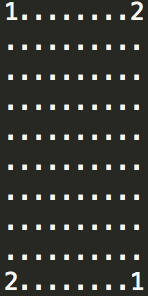
\includegraphics [height=3cm]{example}
\caption{An Extreme Example}
\label{aee}
\end{center}

In order to optimize the algorithm, we come up with three main points:

(1) We can combine some muti-SAT terms together to a mixed term, which can reduce the check time (it can approximately accelerate the speed twice).

(2) It has no meaning if one droplet $d$ takes the squared area, it means the situation

\[
c_{p_1, d} = c_{p_2, d} = c_{p_3, d} = c_{p_4, d} = TRUE
\]

should be forbidden where $p_1 = (x, y)$, $p_2 = (x + 1, y)$, $p_2 = (x, y + 1)$, $p_4 = (x + 1, y + 1)$, Z3 solver will search all the posibilities including this situation. However, under the circumstances of this specific problem, this situation don't contribute any to the final answer. Therefore, we can manually add the \textbf{prune term 1} for each $p$ and $d$ (where $p_1 = p$):

\[
\neg(c_{p_1, d} \wedge c_{p_2, d} \wedge c_{p_3, d} \wedge c_{p_4, d})
\]

(3) when consider the 4 totally empty grid (no obstacle/terminal), for one single droplet, there are 2 ways to pass from the left-down to up-right, just like the Figure \ref{a4v}.

\begin{center}
\makeatletter
\def\@captype{figure}
\makeatother
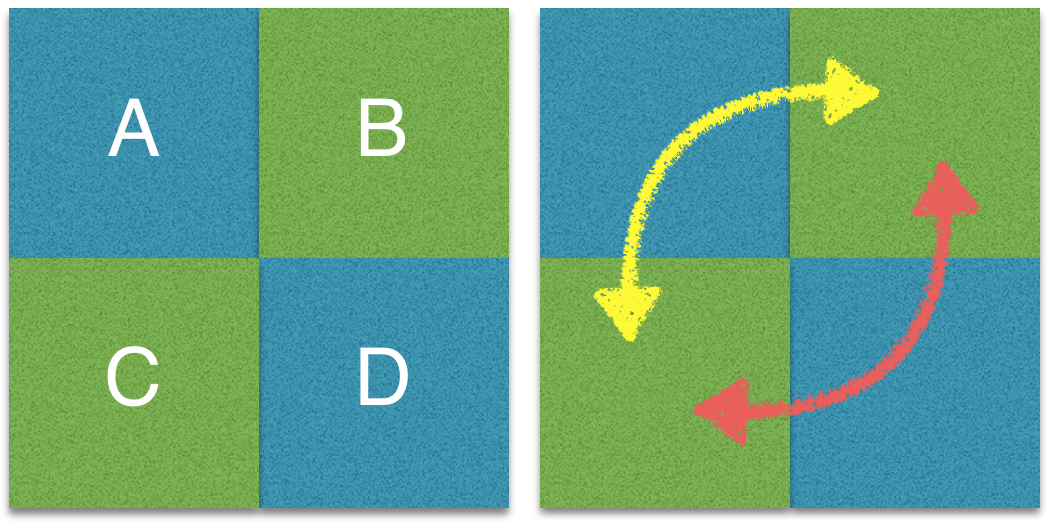
\includegraphics [height=3cm]{example2}
\caption{A 4-Block View}
\label{a4v}
\end{center}

we can find the path C-A-B and C-D-B are both ok, and Z3 solver will check all the 2 path, so we can forbid this situation simply by the following contraint \textbf{prune term 2}(we forbid C-D-B for any $p$ and $d$):

\[
(\sum_{x=1}^{M}{[c_{p_1,x}]} = 0) \to \neg(c_{p_2,d} \wedge c_{p_3,d} \wedge c_{p_4,d})
\]

where $p = p_1 = (x, y)$, $p_2 = (x + 1, y)$, $p_2 = (x, y + 1)$, $p_4 = (x + 1, y + 1)$. Moreover, we can strength the contraint by the following expression if we check other conditions.

\[
(\sum_{x=1}^{M}{[c_{p_1,x}]} = 0) \to \neg(c_{p_2,d} \wedge c_{p_3,d})
\]

and another symmetric terms should also be added (to forbid A-C-D from 2 paths A-C-D and A-B-D)

The prune term 1 and prune term 2 is of great significance, if we use these terms, we can get the answer of example in Figure \ref{aee} in 1.5 seconds.

\section{Results and Evaluation}


\section{System Architecture}

\subsection{Overview}

The whole system architecture can be divide into four main parts

\begin{itemize}
    \item the core part, which consists of the whole algorithm(routingalgo.h, routingalgo.cpp, routing.h, routing.cpp, message.h, message.cpp, routing$\_$test.cpp).
    \item the checker part, which is implemented to check if the answer calculated by the algorithm is legal and correct(checker.h, checker.cpp).
    \item the evaluation part, which is implemented to evaluate the efficiency and correctness of the algorithm(evaluate.h, evaluate.cpp, report.cpp).
    \item the demo part, we develop a simple demo, you can define your own maps in GUI and view the general results and detailed results to better understanding the problem from a dropout perspective (demo.cpp, demo.h, editor.cpp).
\end{itemize}

The makefile file can generate three different executable files

\begin{itemize}
    \item \textbf{make test}: generate a executable file that can choose one/several algorithm to get a answer for a given testcase.
    \item \textbf{make repo}: generate a executable file that evaluates different algorithms.
    \item \textbf{make demo}: generate a executable file that gives a GUI, which you can define the map and run it using a concrete algorithm.
\end{itemize}

We will introduce the four main parts of our system in the following subsection.

\subsection{Core}

The CORE part use a design pattern of strategy, mainly consists of 3 main group of classes

\begin{itemize}
    \item \textbf{RoutingSolver}: make preparations and call the main algorithm
    \item \textbf{RoutingAlgo} and the classes inherit it \textbf{RoutingSatAlgo}, \textbf{RoutingSatAlgoFlow}, \textbf{RoutingSatAlgoFlowPrune}, \textbf{RoutingSatAlgoPointPrune}: it is the main algorithm
    \item \textbf{message}: store the answer of the algorithm
\end{itemize}

Figure \ref{ir1} shows the inheritance relationship of these classes (except class message).

\begin{center}
\makeatletter
\def\@captype{figure}
\makeatother
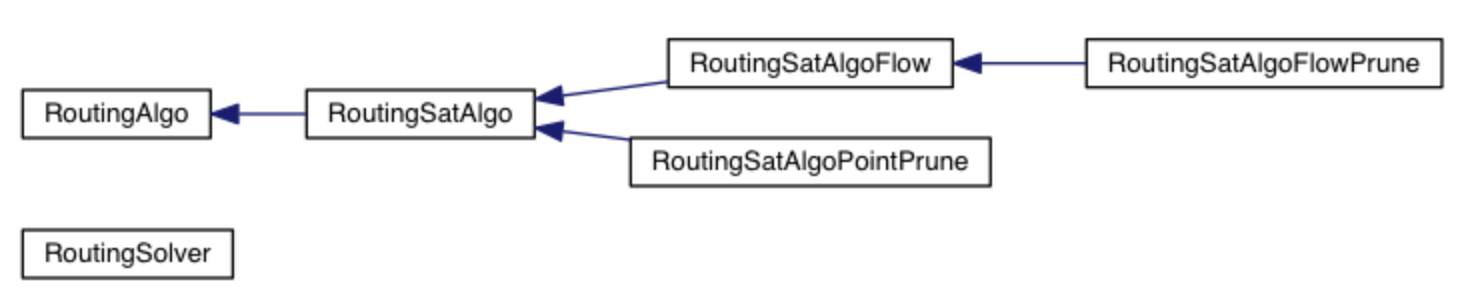
\includegraphics [height=1.5cm]{ir1}
\caption{Inheritance Relationship in Core Part}
\label{ir1}
\end{center}

\textbf{RoutingSolver}'s UML diagram is in Figure \ref{UMLRoutingSolver}, we can see that we must make one algorithm be the composition of RoutingSolver when a RoutingSolver object is created. the function of it's member functions are as follows:

\begin{itemize}
    \item load() : load the vector of string from file
    \item getBlock() : get the map (stored as a matrix) from the file
    \item solver(): main function that load data from file and compute the answer by calling the corresponding algorithm.
    \item solve(): call the algorithm
\end{itemize}

\begin{center}
\makeatletter
\def\@captype{figure}
\makeatother
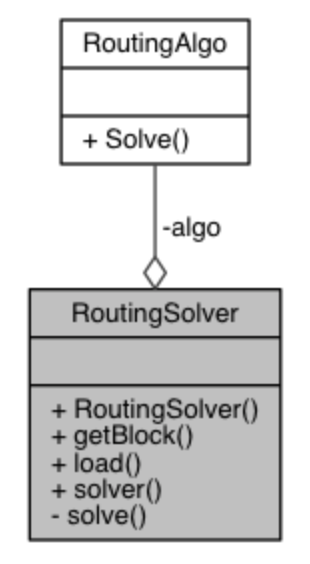
\includegraphics [height=6cm]{UMLRoutingSolver}
\caption{RoutingSolver's UML diagram}
\label{UMLRoutingSolver}
\end{center}

\textbf{RoutingAlgo} is an abstract class of the algorithm, \textbf{RoutingSatAlgo} inherit it and add some common member variables and member functions of sat model, here is the details:

member variable:

\begin{itemize}
    \item sat$\_$context, one, zero are variable for z3 solver. \underline{one} and \underline{zero} is the const expression of integer $1$ and $0$, just for convenience.
    \item n, m, D is the basic information of the board, separately represent the height, width and number of droplets of the board.
\end{itemize}

member funtcion:

\begin{itemize}
    \item GetValue(): this is just an adaptor and converts the expression of z3 to a char ('t' or 'f').
    \item BoolToInt(): convert a bool expression in z3 to a int expression.
    \item GetStartEndPoints(): get the origin and terminal from the board.
    \item GetAns(): get the answer according to the arguments [aug](aug = 0 means get the maximum pairs, aug = 1 means get the minimum length).
\end{itemize}

We just introduce the member variable and member function of class \textbf{RoutingSatAlgoPointPrune} to introduce our structure of algorithm.

\begin{itemize}
    \item idx(), getindx(): get the index of a binary variable(such as $c_{p,d}$), because we use z3::expr$\_$vector(an 1-dim vector) to store the binary variables.
    \item AddSatTerms(): define binary variables of the model.
    \item EstablishModels(): define contraints of the model.
    \item PruneTerms(): add some prune contraints.
    \item FindPath(): find the final path via the results of z3.
\end{itemize}

The Figure \ref{UMLRoutingAlgo} gives an overview of the family of algorithms.

\begin{center}
\makeatletter
\def\@captype{figure}
\makeatother
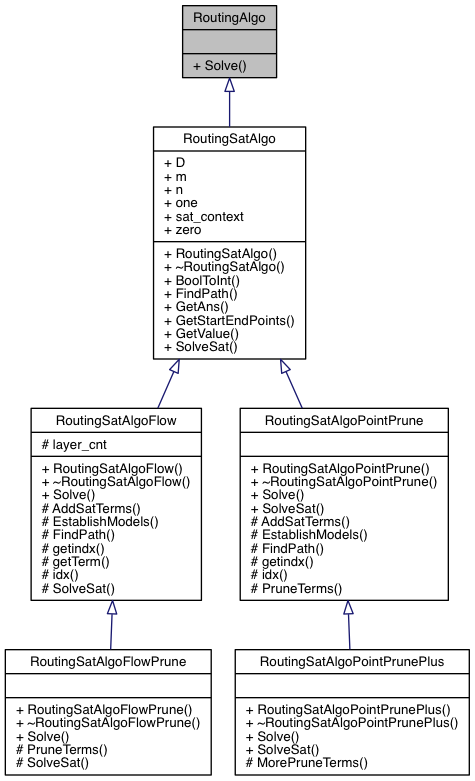
\includegraphics [height=15cm]{UMLRoutingAlgo}
\caption{RoutingAlgo's UML diagram}
\label{UMLRoutingAlgo}
\end{center}

When it comes to the concrete implement of our algorithm, we use the contraints which illustrated in Section 3 and try to combine several expressions to one single expression to reduce the time.

The class \textbf{message} store the answer of the algorithm. 

\begin{itemize}
    \item board, d$\_$, m$\_$, n$\_$: store the main information of the original board.
    \item totlength, totpair: store the total length of the answer and total connected pairs of the answer.
    \item push(): store a new step of droplet $d$.
    \item display(): display the final board(consists of path) and the detailed paths of all connected pairs.
\end{itemize}

Figure \ref{UMLmessage} shows the details of the class.

\begin{center}
\makeatletter
\def\@captype{figure}
\makeatother
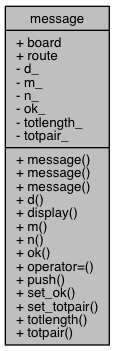
\includegraphics [height=7cm]{UMLmessage}
\caption{message's UML diagram}
\label{UMLmessage}
\end{center}


\subsection{Checker}

The Checker part consists of 2 single classes:

\begin{itemize}
    \item \textbf{CheckerMessage}: store the detailed checker information.
    \item \textbf{AnswerChecker}: check if one answer is legal and correct.
\end{itemize}

In \textbf{CheckerMessage}, \underline{ok} shows if the answer pass the check process and \underline{res} shows the detailed information, Figure \ref{UMLCheckerMessage} shows concrete information.

\begin{center}
\makeatletter
\def\@captype{figure}
\makeatother
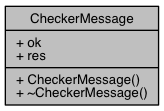
\includegraphics [height=2cm]{UMLCheckerMessage}
\caption{CheckerMessage's UML diagram}
\label{UMLCheckerMessage}
\end{center}

In \textbf{AnswerChecker}, we make 2 kinds of check processes.

\begin{itemize}
    \item legal$\_$check(): check if the given output is legal, we divided this processes into 3 parts, separately implemented in \underline{pairs$\_$check()} (check if the out.totpair is correct), \underline{length$\_$check()} (check if the out.totlength is correct), \underline{legal$\_$step$\_$check()} (check if the step is legal, including checking the origin, terminal and every step).
    \item cmp$\_$check(): check if the answer of [ans] is better than [out], we assume [ans] is a solution that is approximately best, if [out] is worse than [ans], [out] is not the best solution, detailed evaluation method will be illustrated in the next subsection.
\end{itemize}

Figure \ref{UMLAnswerChecker} shows an overview of class AnswerChecker.

\begin{center}
\makeatletter
\def\@captype{figure}
\makeatother
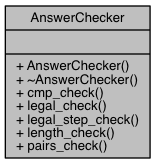
\includegraphics [height=3cm]{UMLAnswerChecker}
\caption{AnswerChecker's UML diagram}
\label{UMLAnswerChecker}
\end{center}

\subsection{Evaluation}

The Evaluation part consists of 3 main class families.

\begin{itemize}
    \item \textbf{DataGenerator} and \textbf{RandomDataGenerator}: they are designed to generate test data.
    \item \textbf{Time}: it is designed to store the time used by a concrete algorithm and analyse in a naive method (calculate the average time used and the standard deviation) to give a summary of the efficiency of the algorithm.
    \item \textbf{Evaluation}: it is designed to evaluate the correctness and efficiency of the algorithm.
\end{itemize}

The class family \textbf{DataGenerator} uses the design pattern of strategy, \textbf{RandomDataGenerator} will generate a random test case if the size of the board ($N$), the number of droplets ($M$), the proportion of obstacles and the random seed are given, Figure \ref{UMLDataGenerator} shows more information:

\begin{center}
\makeatletter
\def\@captype{figure}
\makeatother
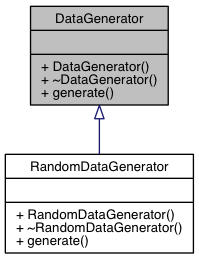
\includegraphics [height=4cm]{UMLDataGenerator}
\caption{DataGenerator's UML diagram}
\label{UMLDataGenerator}
\end{center}

By class \textbf{Time}, we can add a new time span (\underline{push$\_$back()}) and get the summary data(\underline{average()}, \underline{standard$\_$deviation()}) easily, more infomation can be seen in Figure \ref{UMLTime}

\begin{center}
\makeatletter
\def\@captype{figure}
\makeatother
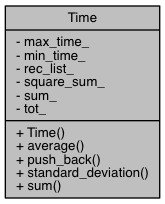
\includegraphics [height=3.5cm]{UMLTime}
\caption{Time's UML diagram}
\label{UMLTime}
\end{center}

Having the tools of data generator, time recorder and checker, we can evaluate our algorithm in the following way:

We can create an object of the class \textbf{Evaluation} to evaluate two specific algorithms by one kind of test data which generated by a specific data generator. We execute the evaluation several times. Therefore, when we create an object of Evaluation, we should give these arguments: algo-a, algo-b, data-generator, the number of test-cases in this evaluation.

For each test case, seed is different, but other arguments are same. After generating the test data, we execute the two algorithms separately and record their use of time, then we check the legality of the answers given by the two algorithms, finally we use cmp$\_$check() in AnswerChecker to check if the answer given by one algorithm is worse than the answer given by another algorithm. Some people think this method might not be useful, but it really works. In our evaluation, even two algorithms all have mistakes, we can also detect the errors and finally fix the bugs. The communication diagram of class Evaluation in Figure \ref{UMLEvaluation} can give an overview:

\begin{center}
\makeatletter
\def\@captype{figure}
\makeatother
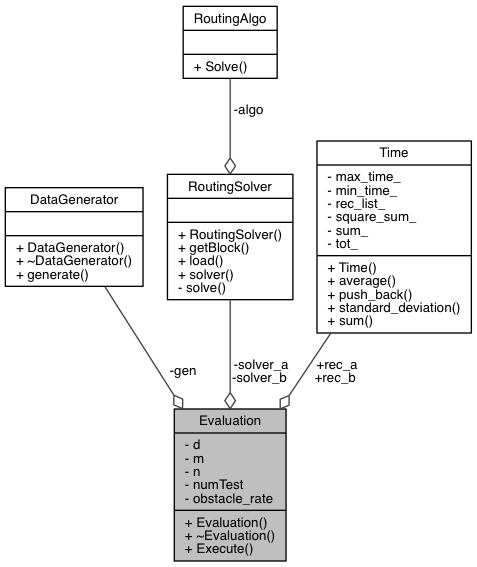
\includegraphics [height=8cm]{UMLEvaluation}
\caption{Evaluation's communication diagram}
\label{UMLEvaluation}
\end{center}

\subsection{Demo}

The demo part uses the design pattern of state and including 2 major class family.

\begin{itemize}
    \item \textbf{State}, which is inherited by 5 classes, and the inheritance relationship is illustrated in Figure \ref{UMLState}.
    \item \textbf{Demo}, uses class State, the state design pattern and a lot of corresponding member variables to give a GUI to the user.
\end{itemize}

\begin{center}
\makeatletter
\def\@captype{figure}
\makeatother
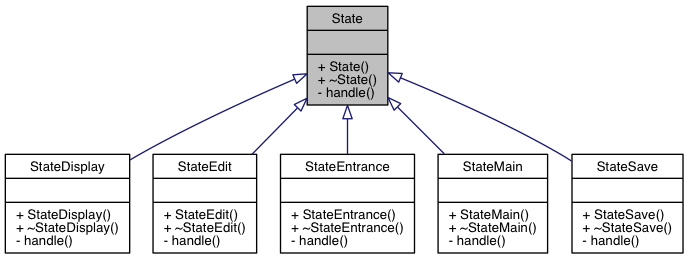
\includegraphics [height=3cm]{UMLState}
\caption{State's inheritance relationship diagram}
\label{UMLState}
\end{center}

As shown above, the class \textbf{State} is inherited by 5 classes, and the functions of the 5 classes are as followings.

\begin{itemize}
    \item \textbf{StateEntrance}: the state of entrance interface, let user to define the size of the map.
    \item \textbf{StateMain}: the state of main interface, user can view the map, save the map, edit the map or let the algorithm calculate the answer.
    \item \textbf{StateEdit}: the state of edit interface, user can edit the map: move the cursor by w/a/s/d; enter '1' - '9' to add terminals; enter 'o' to add obstacles.
    \item \textbf{StateSave}: the state of save interface, user can enter the filename of the map
    \item \textbf{StateDisplay}: the state of display interface, user can view the answer and see how droplets path to get further understanding of the idea of droplet
\end{itemize}

We can see how the class \textbf{Demo} organize all the things together by seeing the following communication diagram of it in Figure \ref{UMLDemo}

\begin{center}
\makeatletter
\def\@captype{figure}
\makeatother
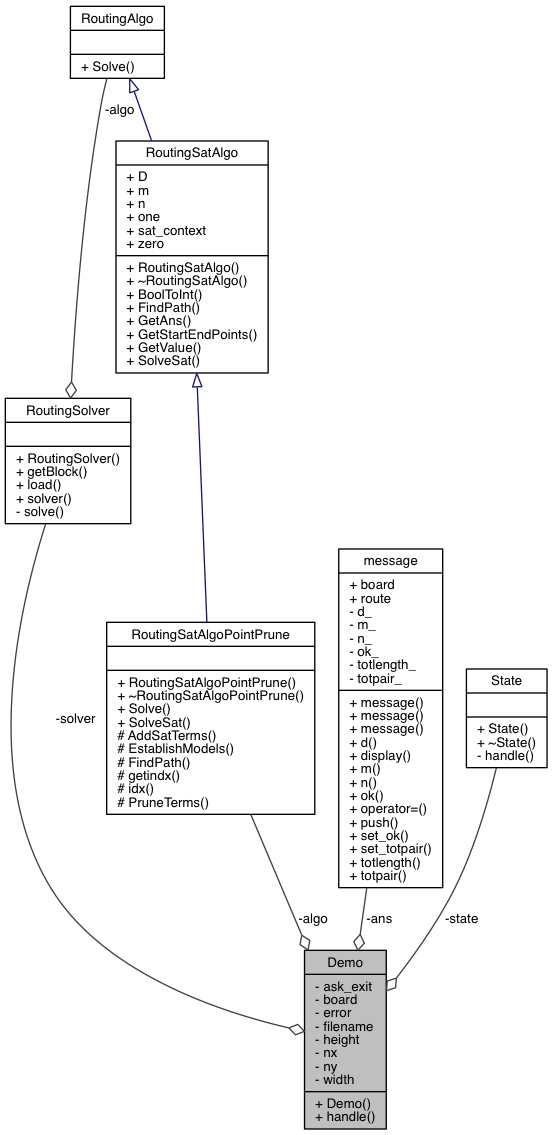
\includegraphics [height=12cm]{UMLDemo}
\caption{Demo's communication diagram}
\label{UMLDemo}
\end{center}

\section{Data Flow}

We describe out data flow using the example of 3 executable files shown in the previous section.

\subsection{Test}

In the beginning, the object of one particular routing algorithm (the class which inherit the class \textbf{RoutingAlgo})is created, and we use it's address as a pointer to create the object of \textbf{RoutingSolver}.

Afterwards, we send a \underline{string} to the object \textbf{RoutingSolver} and it calls the function load() to get the map, then it convert the map, which in form of \underline{vector<string>}, to the objective form \underline{vector<vector<int> >}, and use it, the size of the board (two \underline{int}egers) and the number of pairs (one \underline{int}eger) as parameters to call the main function Solve() in a concrete \textbf{RoutingAlgo} object.

The function Solve() firstly add an [aug] = 0 and calls the function SolveSat(), which means the object is to find the solution with largest number of pairs. In the main process of SolveSat(), we create \underline{expr$\_$vector} as binary variables and call the functions AddSatTerms(), EstabishModels(), PruneTerms() successively to build the model, it use GetAns() to check if it should calulate the minimum length (set [aug] = 1 and recall the function SolveSat()), and finally calls the function FindPath() to return a \textbf{message} as a result.

Therefore, it receives a \textbf{message} variable that returns the ans of the given map.

Afterwards, it uses function getBlock() in \textbf{RoutingSolver} to get the map in form of \underline{vector<vector<int> >} and put the map(\underline{vector<vector<int> >}) and the ans(\underline{message}) as parameters to the function legal\_check in the object of \textbf{AnswerChecker} to check if the ans is legal, after many turns of check, it returns an object of \textbf{CheckerMessage} as a result of checker.

\subsection{Report}

In the beginning, it creates the objects of two diffent implementation of the abstract class \textbf{RoutingAlgo} and one object of the implementation of the abstact class \textbf{DataGenerator}, and use the addresses of these objects as pointer to create an object of \textbf{Evaluation}. (Meanwhile, it should send the arguments that decide the type of the test data)

Afterwards, it calls the function execute() in the object of \textbf{Evaluation}. Therefore, for each test, it uses the arguments which describe the data type as parameter to call the data generator to generate one single test. Then it uses the way described in the previous subsection to get the two answer and check it, meanwhile it calculate the time they used separately and send it to the composition object \textbf{Time} in class \textbf{Evaluation}.

Finally, we can print out the detailed information stored in the object \textbf{Time}.

You can also refer to the communication diagram of class \textbf{Evaluation} for better understanding in Figure \ref{UMLEvaluation}

\subsection{Demo}

The data flow is quite obvious in the part of demo and you can refer to both the communication diagram of class \textbf{Demo} in Figure \ref{UMLDemo} and the next section for better understanding.

\section{Tutorial for GUI}

We also develop a GUI to let the user define their own map, and here is a simple tutorial.

Firstly, compile it and call the executable file.

\begin{lstlisting}
$ make edit
$ ./editor
\end{lstlisting}

then you enter the entrance interface, you should enter the size of the board (like Figure \ref{ge}):

\begin{center}
\makeatletter
\def\@captype{figure}
\makeatother
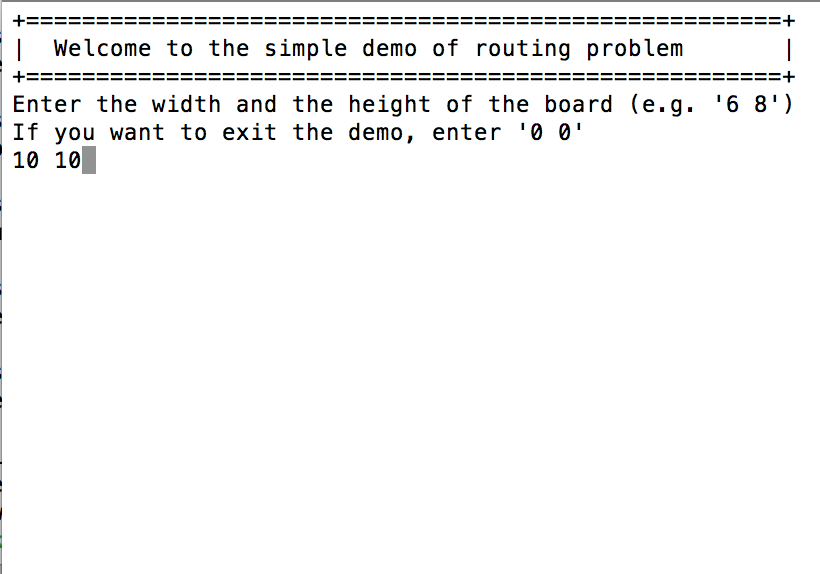
\includegraphics [width = 9cm]{GUI-entrance}
\caption{GUI: Entrance Interface}
\label{ge}
\end{center}

Press 'Enter' and you will see the main interface in Figure \ref{gi}

\begin{center}
\makeatletter
\def\@captype{figure}
\makeatother
\includegraphics [width = 9cm]{Gui-main}
\caption{GUI: Main Interface}
\label{gi}
\end{center}

Press 'i' to enter the editor interface, and use key 'w/a/s/d', '0' ~ '9' and 'o' to edit the map, and then press 'x' to return to the main interface (Figure \ref{ged} shows the edit interface)

\begin{center}
\makeatletter
\def\@captype{figure}
\makeatother
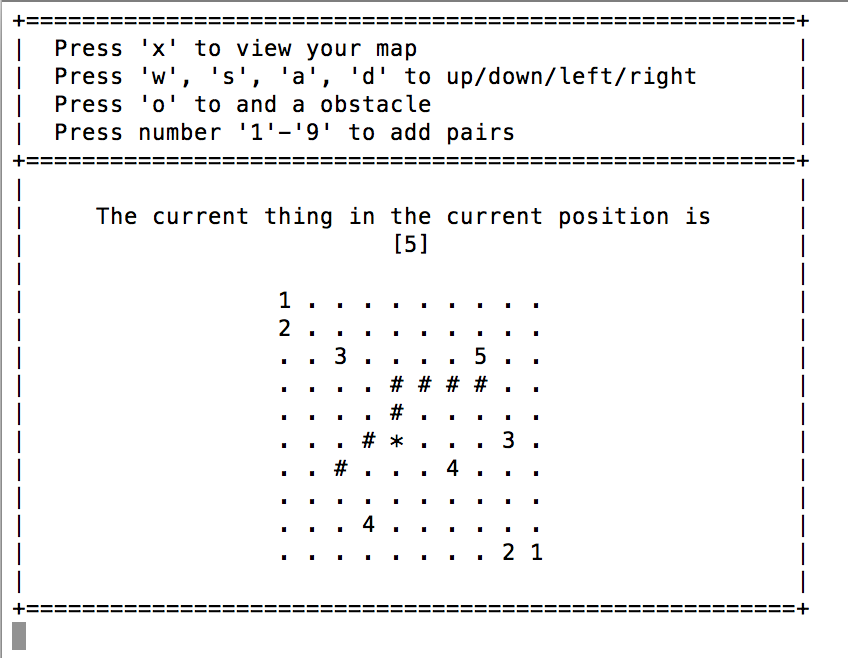
\includegraphics [width = 9cm]{GUI-edit}
\caption{GUI: Edit Interface}
\label{ged}
\end{center}

Then press 's' to save the file.

\begin{center}
\makeatletter
\def\@captype{figure}
\makeatother
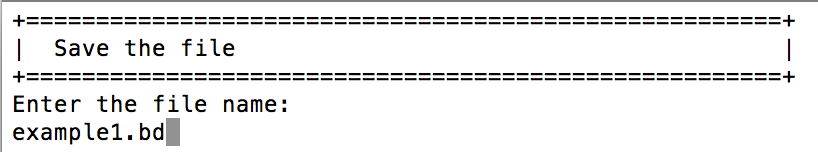
\includegraphics [width = 9cm]{GUI-save}
\caption{GUI: Save Interface}
\label{gs}
\end{center}

Afterwards, when returned to the main interface, press 'e' to let algorithm to calculate the answer. And you will see the interface like this in Figure \ref{gex}

\begin{center}
\makeatletter
\def\@captype{figure}
\makeatother
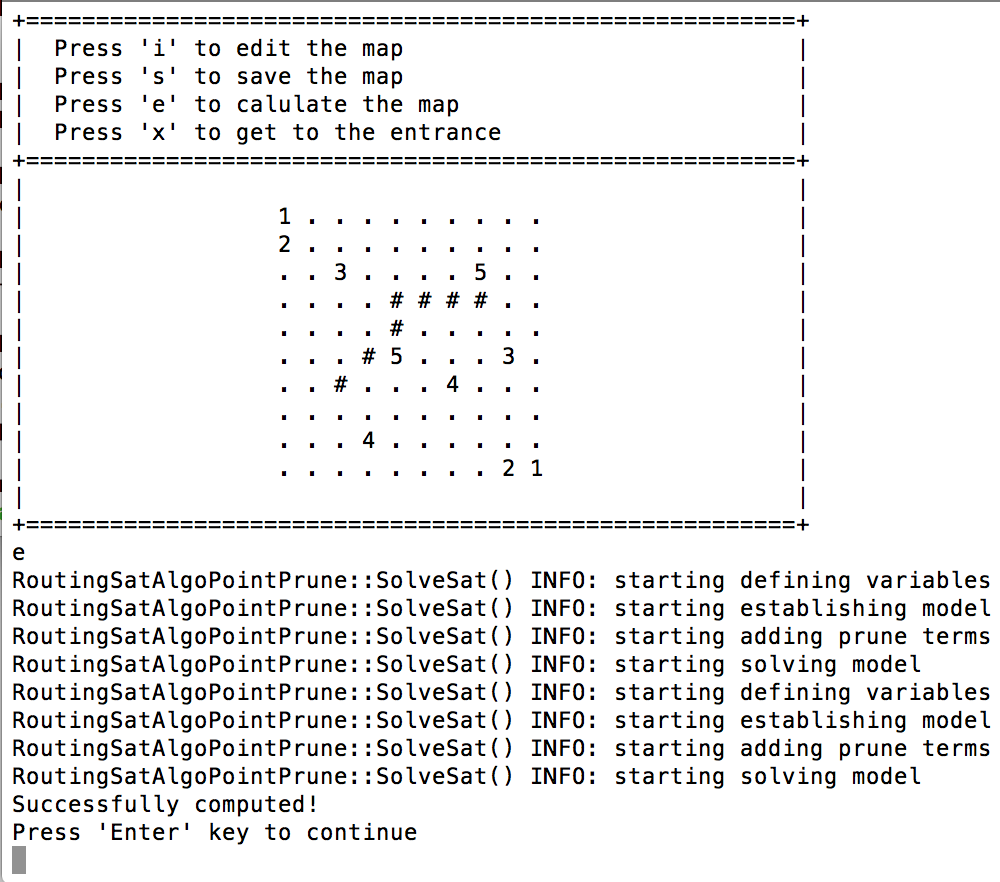
\includegraphics [width = 9cm]{GUI-execute}
\caption{GUI: Main Interface After Executed}
\label{gex}
\end{center}

Finally, press 'Enter' to enter the display interface, you can press '1' ~ '5' to see more detailed infomation about each droplet (see how they step the path separately).

\begin{center}
\makeatletter
\def\@captype{figure}
\makeatother
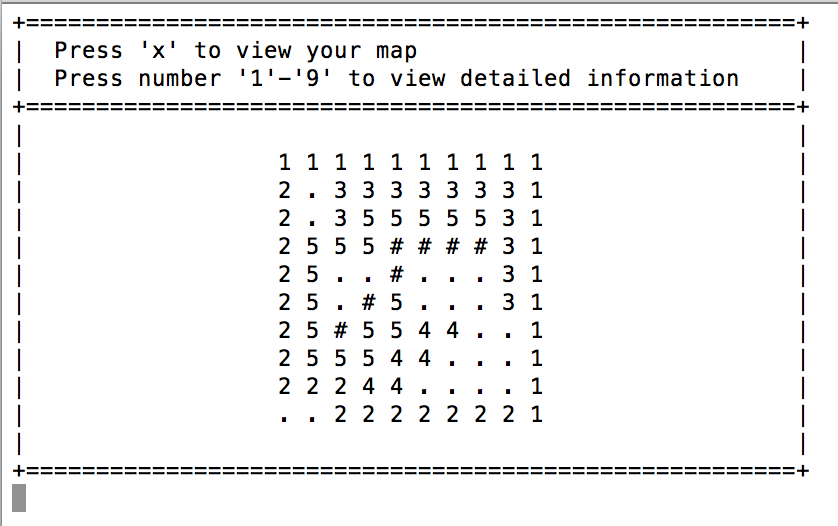
\includegraphics [width = 9cm]{GUI-display}
\caption{GUI: Display Interface}
\label{gd}
\end{center}


\begin{thebibliography}{1}
\bibitem{source1}
Oliver Keszocze, Robert Wille, Krishnendu Chakrabarty, Rolf Drechsler. A General and Exact Routing Methodology for Digital Microfluidic Biochips.
\bibitem{source2}
Leonardo De Moura and Nikolaj Bjørner. Z3: An efficient SMT solver. In Tools and Algorithms for the Construction and Analy- sis of Systems, pages 337–340. Springer, 2008. Z3 is available at http://z3.codeplex.com/.
\end{thebibliography}


\end{document}

